\documentclass[twocolumn]{article}
\usepackage{graphicx}
\usepackage{caption}
\usepackage{subfigure}
\usepackage[pdfborder={0 0 0},plainpages=false]{hyperref}
\usepackage{url}
\usepackage{tikz}
\usetikzlibrary{shapes,arrows,automata}

\title{Bachelor project proposal}
\author{Chiel de Roest\\4036832 \and Harmjan Treep\\4011724}
\date{}

\begin{document}

\maketitle

\begin{figure*}[t]
	\subfigure{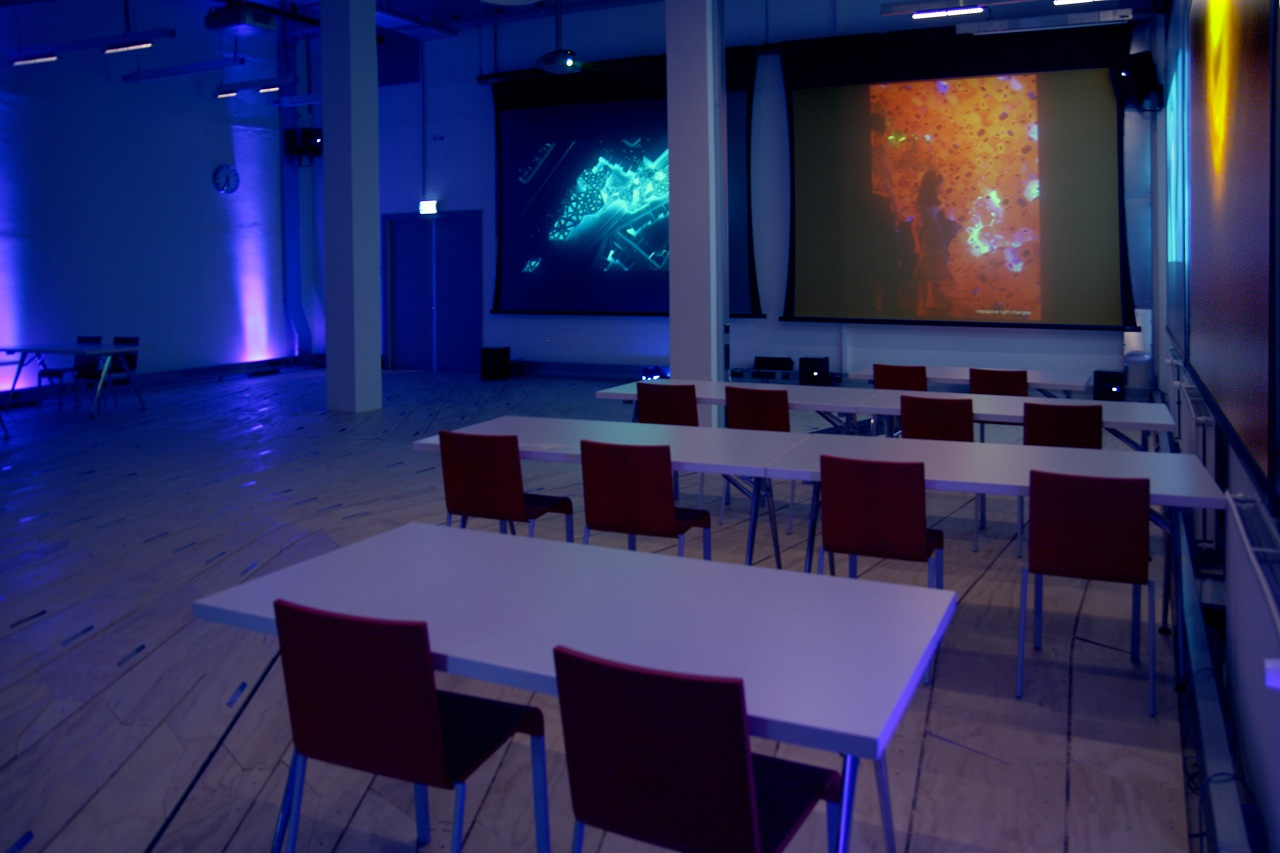
\includegraphics[width=\columnwidth]{protospace}}~
	\subfigure{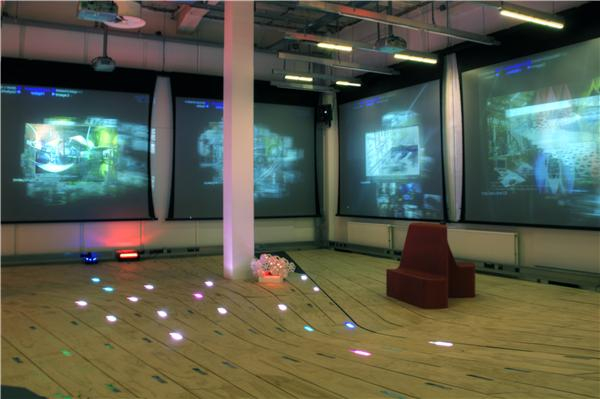
\includegraphics[width=\columnwidth]{protospace2}}~
	\caption{The protoSPACE 3.0 room}
	\label{fig:protospace}
\end{figure*}

\section*{Problem}
	The hyperbody research group (\url{http://www.hyperbody.bk.tudelft.nl/}) in faculty of Architecture has the goal to
	\begin{quote}
		explore techniques and methods for designing and building of non-standard, virtual and interactive architectures.
	\end{quote}
	A room in the faculty of Architecture has been equipped with a floor with nodes in it.
	Each of these nodes has a RGB LED and a pressure sensor.
	This room is called protoSPACE 3.0 as seen in Figure \ref{fig:protospace}.
	
	Every tile in the floor has its own processor.
	Every processor can only talk to its direct neighbours.
	Advantages of this is that you can just add new tiles with the code deployed on them and they will seamlessly integrate into the floor.
	Traditionally you would do this with a central server who controlls all the LEDs.
	From a certain size however one central server cannot handle the load.
	This is why sensor node technology is a solution.
	Even if you could implement the protoSPACE 3.0 floor without sensor nodes, with sensor nodes you can extend the floor infinitly without problems.
	Since the floor is a prototype there is one communication bus where all nodes are connected to, the CAN bus.
	The system is displayed in Figure \ref{fig:network}.
	The CAN bus is the red line and every node can talk to its neighbours via the black arrows.
	
	\begin{figure}[t]
		\centering
		\tikzstyle{square}=[rectangle,thick,minimum size=0.5cm,draw=blue!80,fill=blue!20]
		\begin{tikzpicture}[auto, outer sep=3pt, node distance=2cm,>=latex']
			\node [square] (1) {Node 1};
			\node [square] (2) [right of=1] {Node 2};
			\node [square] (3) [right of=2]{Node 3};
			\node [square] (4) [below of=1]{Node 4};
			\node [square] (5) [right of=4]{Node 5};
			\node [square] (6) [right of=5]{Node 6};
			\node [square] (7) [below of=4]{Node 7};
			\node [square] (8) [right of=7]{Node 8};
			\node [square] (9) [right of=8]{Node 9};
			
			\draw [<->,thick] (1) --  node {} (2) ;
			\draw [<->,thick] (2) --  node {} (3) ;
			\draw [<->,thick] (1) --  node {} (4) ;
			\draw [<->,thick] (2) --  node {} (5) ;
			\draw [<->,thick] (3) --  node {} (6) ;
			\draw [<->,thick] (4) --  node {} (5) ;
			\draw [<->,thick] (5) --  node {} (6) ;
			\draw [<->,thick] (4) --  node {} (7) ;
			\draw [<->,thick] (5) --  node {} (8) ;
			\draw [<->,thick] (6) --  node {} (9) ;
			\draw [<->,thick] (7) --  node {} (8) ;
			\draw [<->,thick] (8) --  node {} (9) ;
			
			\path[red,thick] (7) edge [bend left] node {} (4)
			      (4) edge [bend left] node {} (1)
			      (1) edge [bend left] node {} (2)
			      (2) edge [bend right] node {} (5)
			      (5) edge [bend right] node {} (8)
			      (8) edge [bend right] node {} (9)
			      (9) edge [bend left] node {} (6)
			      (6) edge [bend left] node {} (3);
		\end{tikzpicture}
		\caption{A sensor node network with a CAN bus}
		\label{fig:network}
	\end{figure}
	
	The role of the Embedded Systems group in this effort is to research effective ways of implementing a node network which is easy to extend and program.
	The protoSPACE 3.0 room is already designed and produced, but still no effective way of programming and debugging is in place making writing code for the room a very tedious task.
	
	We want to do our bachelor thesis with the Embedded Systems group and work on the toolchain features such as programming and debugging a node network.

\section*{Proposal}
	What we want to focus on for our bachelor project is programming individual nodes and the entire network over the CAN bus.
	Right now if you want to flash the entire network you have to go from node to node with your programmer.
	We want to develop a tool to flash a node.
	This could be done with a virtual machine in which we load code over the CAN bus, the department has experience with proto and eLua.
	We could also try to implement a CAN bootloader on the hardware.
	This a point of research in our assignment.
	
	An extension of our assigment is distributed programming, so you give your code to a node which then updates all neighbours untill every node has the new code.
	The CAN bus is handy because you can address a single node in the network, for debugging purposes, but in real life in large networks you just want to flash an entire network without having a CAN bus run through all nodes.
	
	To make this more clear we tried to compile a set of tasks we would have to accomplish.
	\begin{itemize}
		\item Familiarize ourselves in protoSPACE 3.0 hardware, which is:
		\begin{itemize}
			\item The LPCXpresso 1769
			\item Extra board the LPCXpresso 1769 is tagged on
			\item The UART protocol for communication between nodes
			\item The CAN protocol for monitoring and programming nodes
		\end{itemize}
		\item Design the software to program the nodes
		\item Implement the program
		\item Couple our program with a GUI
		\item Showcase our findings with an application
	\end{itemize}
	
	We think this is a challenging assignment.
	With our current knowledge is it hard to estimate how long we would need to implement such a system.
	We do however think we should be able to implement programming the nodes over the CAN bus, and if we do finish that before the end of the project we can focus on an application in protoSPACE 3.0.
	
	We will be supervised by Stefan Dulman (\url{http://www.st.ewi.tudelft.nl/~dulman/}).
	We can also get support from the master students in his research group.

\end{document}
